\documentclass[a4paper, oneside]{discothesis}

\usepackage[utf8]{inputenc}
\usepackage[T1]{fontenc}
\usepackage{graphicx}
\usepackage{epstopdf}
\usepackage{epigraph}
\usepackage{amsmath}

\thesistype{Master's Thesis}
\title{Rethinking Adversarial Examples}

\author{Yahya Jabary}
\email{yjabary@ethz.ch}

\institute{Computer Engineering and Networks Laboratory \\[2pt] ETH Zürich}

% \logo{
\includegraphics[width=0.2\columnwidth]{figures/dsg-logo}}

\supervisors{Prof.\ Dr.\ Roger Wattenhofer\\[2pt] Prof.\ Dr.\ Schahram Dustdar}

\keywords{Robustness, Alignment, Interpretability, Algorithmic Models}
% \categories{ACM categories go here.}

\date{\today}

%
% extended config
%

\usepackage{mathtools}

\setlength\parindent{0pt}

% example boxes
% https://www.overleaf.com/latex/examples/simple-stylish-box-design/stzmmcshxdng
\usepackage[many]{tcolorbox}
\usepackage{mathspec}
\usepackage{setspace}
\usepackage{multicol}
\tcbset{sharp corners, colback = white, before skip = 0.5cm, after skip = 0.5cm, breakable}
\newtcolorbox{highlightbox}{sharpish corners, boxrule = 0pt, leftrule = 4.5pt, enhanced, breakable, fuzzy shadow = {0pt}{-2pt}{-0.5pt}{0.5pt}{black!35}}

%
% content
%

\begin{document}

\frontmatter % do not remove this line
\maketitle

\cleardoublepage

\begin{acknowledgements}
	This thesis comes from working on a problem that truly matters to me, in an environment where curiosity and passion were shared, and I felt a sense of belonging. The topic of adversarial examples reflects my journey well, highlighting how subtle differences in perspective can lead to vastly different interpretations and outcomes.

	I'm deeply grateful to those who supported me along the way. My parents, Shima and Florian, and my family, for their unwavering support, even when I took risks and turned down financial opportunities to pursue my passion. My partner, Laura, whose love and encouragement crossed the Atlantic and got me through many long nights.
	
	I owe much to those who made this work possible. Prof.\ Wattenhofer, for trusting me with this project and guiding me with wisdom and humor. Andreas Plesner, who was just as much of a mentor as a collaborator, for his dedication to our vision. Turlan Kuzhagaliyev and Alireza Furutanpey, for their camaraderie.
	
	Thanks also to those whose paths have diverged from mine but whose impact remains with me: Prof.\ Schahram Dustdar, who enabled my studies abroad, and Prof.\ Ali Mashtizadeh, who introduced me to operating systems research.
	
	I hope to continue this journey with the same spirit that brought me here.
\end{acknowledgements}

\begin{abstract}
    % The abstract should be short, stating what you did and what the most important result is.
	...
\end{abstract}

\tableofcontents

\mainmatter % do not remove

\chapter{Introduction}

% good style: https://arxiv.org/pdf/2202.02435

We have two goals in writing this document. One: fulfilling the requirements for a master's degree by presenting and extending our original research~\cite{jabary2024seeing} in thesis form. Two: offering a fresh and cohesive perspective on the rapidly evolving and, in our view, really exciting field of adversarial machine learning to a broader audience, with fewer technical prerequisites. We hope it will be valuable to those interested.

\section{Definition}

Adversarial examples are closely related to the concept of perturbation methods.

The origin of perturbations can be traced back to the early days of computational geometry by Seidel et al. in 1998~\cite{seidel1998nature}. Perturbation techniques in computational geometry address a fundamental challenge: handling ``degeneracies'' in geometric algorithms. These are special cases that occur when geometric primitives align in ways that break the general position assumptions the algorithms rely on.

\begin{highlightbox}
	\textbf{Example:} Perturbation scheme for a linear classifier. \\

	Consider a simple case of determining whether a point lies above or below a line~\cite{de2000computational}. While this classification appears straightforward, numerical issues arise when the point lies exactly on the line. Such degeneracies can cascade into algorithm failures or inconsistent results. The elegant solution is to imagine slightly moving (perturbing) the geometric objects to eliminate these special cases. Formally, we can express symbolic perturbation as $p_\varepsilon(x) = x + \varepsilon \cdot \delta(x)$ where $x$ is the original input, $\varepsilon$ is an infinitesimally small positive number the exact value of which is unimportant, and $\delta(x)$ is the perturbation function to break degeneracies. \\

	A perturbation scheme should be (1) consistent, meaning that the same input always produces the same perturbed output (2) infinitesimal, such that perturbations are small enough not to affect non-degenerate cases and (3) effective, in breaking all possible degeneracies. \\

	One powerful perturbation approach is Simulation of Simplicity (SoS)~\cite{franklin2022implementing, edelsbrunner2002topological, edelsbrunner2001sink, edelsbrunner1990simulation, levy2016robustness, schorn1993axiomatic}. SoS systematically perturbs input coordinates using powers of a symbolic infinitesimal. For a point $p_i = (x_i, y_i)$, the perturbed coordinates become:

	$$(\tilde{x_i}, \tilde{y_i}) = (x_i + \varepsilon^{2i}, y_i + \varepsilon^{2i+1}) = p_i + \varepsilon^{2i} \cdot (1, \varepsilon)$$

	This scheme ensures that no two perturbed points share any coordinate, effectively eliminating collinearity and other degeneracies.
\end{highlightbox}

The beauty of perturbation methods lies in their ability to handle degeneracies without explicitly detecting them, making geometric algorithms both simpler and more robust.

Adversarial examples on the other hand, first introduced by Szegedy et al. in 2014~\cite{szegedy2013intriguing}, follow the same principles as perturbation methods, but with the opposite objective. Instead of seeking to eliminate degeneracies (brittleness in the decision boundary), they exploit them to cause targeted misclassifications. Intuitively they can be understood as seeking the closest point in the input space that lies on the ``wrong side'' of a decision boundary relative to the original input. This shift, applied to the original input, creates an adversarial example.

\begin{highlightbox}
	\textbf{Example:} Fast Gradient Sign Method (FGSM) \\

	FGSM is one of the earliest and most widely recognized adversarial attack techniques, introduced by Goodfellow et al.~\cite{goodfellow2014explaining} in the context of visual recognition tasks. Given an input image $x$, FGSM generates an adversarial example $x'$ by perturbing the input in the direction of the gradient of the loss function with respect to the input.\\

	The perturbation is controlled by a parameter $\varepsilon > 0$~\footnote{Commonly $\varepsilon = 8/255$ for 8-bit images, so it stays within the precision constraints of the pixel values.}, which determines the magnitude of the change based on the direction of change for each pixel or feature in the input $x$. The model's loss function denoted by $J$, $\theta$ represents the model's parameters, and $y$ is the true target label. \\
	
	It works by calculating the gradient of the loss function with respect to the input, $\nabla_x J(\theta, x, y)$, and then adjusting the input in the direction of this gradient. The sign of the gradient, $\text{sign}(\nabla_x J(\theta, x, y))$, is used to ensure that the perturbation is small, while the $\ell_\infty$-norm constraint ensures that the change to the input remains ``imperceptible'' to human observers~\cite{goodfellow2014explaining, zhang2019adversarial}. More on the concept of imperceptibility later.\\
	
	The process for generating an adversarial example with FGSM can be expressed as:
	
	$$x' = x + \underbracket{\varepsilon \cdot \text{sign}(\nabla_x J(\theta, x, y))}_{\text{Perturbation}}$$
	
	In the untargeted version, the perturbation is designed to increase the loss for the correct class. In the targeted version the perturbation is designed to minimize the loss with respect to the adversary's chosen target class, making the model predict it deliberately.
\end{highlightbox}

While initially discovered in computer vision applications, the attack can be crafted for any domain or data type, even graphs~\cite{Kashyap2024AdversarialAA}. Natural language processing models can be attacked by circumventing the discrete nature of text data~\cite{Han2022TextAA, meng2020geometry, yang2024assessing}. One particularly entertaining example is the subversion of the conference paper-reviewer assignment model by Eisenhofer et al.~\cite{eisenhofer2023no}, where authors preselect reviewers to gain a competitive advantage. Speech recognition systems are vulnerable to audio-based attacks, where crafted noise can cause system failure~\cite{rajaratnam2018noise}. Deep reinforcement learning applications, including pathfinding and robot control, have also shown susceptibility to adversarial manipulations that can compromise their decision-making capabilities~\cite{Bai2018AdversarialEC}.

\section{Types of Adversarial Examples}

Having established the general concept of adversarial examples, we can now explore the various ways they can be categorized. Our system is not exhaustive: The field continues to evolve, with new attack vectors emerging regularly~\cite{Khaleel2024AdversarialAI}.

We can differentiate between white-box and black-box attacks. White-box attacks assume complete knowledge of and access to the target model, while black-box attacks operate with limited or no access to the model's internal workings~\cite{capozzi2024adversarial}. Interestingly, research has shown that in some cases, black-box attacks can be more effective than white-box approaches at compromising model security~\cite{capozzi2024adversarial}.

An attack can be targeted or untargeted. Targeted attacks aim to manipulate the model into producing a specific, predetermined output, whereas untargeted attacks simply seek to cause any misclassification or erroneous output~\cite{capozzi2024adversarial, Kashyap2024AdversarialAA}. This distinction is particularly relevant in security-critical applications, where the attacker's goals may vary from causing general disruption to achieving specific malicious outcomes.

The method used to generate adversarial examples can be gradient-based, optimization-based or search-based strategies. For example, some text-based attacks leverage language models to generate alternatives for masked tokens, ensuring grammatical correctness and semantic coherence~\cite{garg2020bae}.

The extent to which adversarial examples are transferable \textendash{} meaning their ability to fool multiple different models \textendash{} is another way to differentiate them. Some adversarial examples demonstrate high transferability across various model architectures, while others are more model-specific in their effectiveness~\cite{Li2022ASO, li2022review}. Recent research has shown that adversarial examples are more readily transferable between vanilla neural networks than between defended ones~\cite{li2019nattack, zheng2023black}.

Finally, the attacks can be either focused on preserving the semantic meaning of inputs or exploit the mathematical properties of models without regard for semantic interpretation provides~\cite{browne2020semantics}.

\section{Semantics Preservation}

Initially, Szegedy and colleagues proposed using epsilon-bounded perturbations in pixel space to create changes ``imperceptible [to humans]'', that could fool neural networks~\cite{szegedy2013intriguing}. However, the term ``imperceptibility'' is indeed more accurately described as ``semantics preserving'' as demonstrated by recent work~\cite{kariyappasemantics}. The assumption that limiting pixel-space modifications ensures semantic preservation is fundamentally flawed, because substantial pixel-space changes can occur without affecting semantic meaning, such as changes in lighting, exposure, sharpness, angle, shadow, field of view, ..., or the the orientation of an animal's fur~\ref{fig:latentspace}.

Also, assuming that a human under time constraints is fooled by an adversarial example

Additionally, the transferability of adversarial examples to human perception under time constraints raises profound questions about the nature of neural network vulnerabilities. This observation aligns with the perspective that neural network depth might correlate with human processing time, suggesting a deeper connection between artificial and human visual processing systems.

The challenge of defining semantics remains central to this discussion. Without perfect representations that align with human judgment functions, we must rely on the best available encoders as proxies for semantic preservation~\cite{herel2023preserving}. This pragmatic approach acknowledges the limitations of current technology while striving for more meaningful adversarial examples.

Recent work has shown that many generated adversarial examples fail to preserve semantics, with up to 70\% of examples potentially requiring rejection~\cite{herel2023preserving}. This finding emphasizes the importance of developing better methods for ensuring semantic preservation in adversarial attacks, leading to new approaches like Semantics-Preserving-Encoder (SPE) and other manifold-based techniques~\cite{lee2020semantics}.

Moving forward, the field should continue to prioritize semantic preservation over simple pixel-space constraints, acknowledging that true imperceptibility requires a deeper understanding of semantic representation in both human and machine perception systems.





write a paper in a casual but academic tone. write full sentences. don't use enumerations, itemizations, headings. use academic papers as citations.

```
In the paper where adversarial examples are introduced by Szegedy, he says that they're using an epsilon value to limit the changes in the pixel-space, in order to ensure ``imperceptibility [to humans]'', however this doesn't make sense.

first of all the term ``imperceptibility'' here is interchangable with the much more well-defined term ``semantics preserving''.

second of all you can't preserve semantics through changes in the pixel space, because: (1) you can have very few pixels changed and still have a change in semantics, in time constrained humans and the authors didn't conduct any experiments with humans and this constraint doesn't ensure anything and (2) you can have much more pixsels changed and have no change in the semantic space (i.e. changing exposure, sharpness, brightness, angle, shadow, field of view, ... the orientation of the fur of a pet).

recent experiments on the transferability of adversarial examples to the human vision system might sugegst that the core assumptions under which adversarial examples were introduced are flawed, because these attacks do transfer to time constrained humans. this raises the philosophical question of whether it's then justified for a model to be fooled by an attack by which time constrained humans are fooled and whether or what kinds of flaws of the human judgement function we are learning should be learned by the model. this is particularly interesting because ilya sutskever briefly mentions in an interview that he believes an increased depth in a neural network is equivalent to a human with more ``time'' available to perceive something. so this would in some sense further underline.

in order order to be able to decide whether an attack is semantically preserving or not, we need to have a clear definition of what semantics are. in the paper ``what makes an image realistic'' by theis this is discussed further, but in short, as long as we don't have representations that perfectly align with the human judgement function, we can't have a clear definition of what semantics are and to which extent our attacks are working as intended.

therefore for the remainder of this paper we will use the term ``semantics preserving'' instead of ``imperceptibility'' and we refer to the best possible encoder we have at our disposal because we can't have a perfect representation of the human judgement function and did not conduct any experiments with humans.
```

idea: adversarial examples are a problem of misaligned internal representations and not necessarily a problem of attack vectors.

```
having introduced the concepts of an ``Image Space'' a subset of which are reasonably realistic images, a ``latent space'' of how an encoder's latent representations are stored, the reader might reasonably ask why adversarial examples exist to begin with and why the ``latent space'' isn't an accurate depiction of the ``semantic space'' such that our encoder and internal latent representation is entirely undisturbed by any non-semantics-changing perturbations.

we believe that this is further evident by the fact that adversarial exampels transfer across models, datasets, architectures, training procedures. the reason adversarial exampels transfer across models, is because the human visual system they're trying to approximate is, we assume, the same. this is there the theory of platonic representations comes in, that are shared both across modailities (text, image) and models, independent of their architecture, when you take certain slices.

we believe that in it's essence any adversarial vulnerability is therefore not necessarily a vulnerability to attack vectors but just an insufficiently aligned model and a problem of misaligned internal representations. this drift between the human judgement function that the models are trying to learn and the model's internal representation is what causes adversarial examples to exist. this is called the ``human-machine vision gap'' and this is why we believe that the term ``alignment'' is a much more accurate term to describe the problem of adversarial examples, and that the term ``robustness'' is a much more accurate term to describe the solution to this problem.

we make the bold claim that therefore hypothetically, a correctly robustified model that can withstand adversarial attacks is infact a simply better generalizing model to downstream tasks, although it might perform worse on the test set (this is described as the bias-variance tradeoff). our second claim is that therefore the robustness-accuracy tradeoff is a false dichotomy and that it's essentially the same as the bias-variance tradeoff.

therefore what we're studying here isn't necessarily adversarial examples but the human-machine vision gap and the alignment of the model's internal representation with the human judgement function. this is why we believe that the term ``adversarial examples'' is a misnomer and that the term ``misaligned examples'' is a much more accurate term to describe the problem of insufficiently generalizing models.

but it doesn't stop here.
```


idea: transferability to humans



idea: transferability across models


% philosophically speaking the semantic space is the latent space of the human and all models are trying to approximate this platonic space but that's beyond the scope of this thesis.



figure~\ref{fig:latentspace}

realism: \cite{theis2024makes}




\begin{figure}
    \centering
    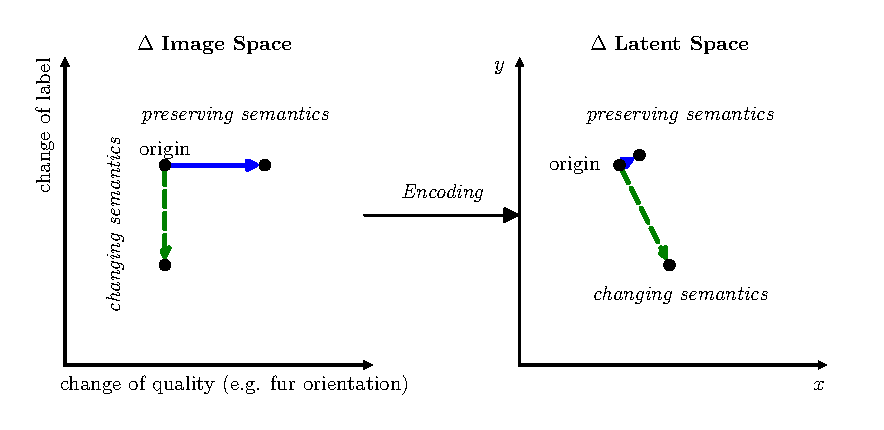
\includegraphics[width=1\columnwidth]{figures/latentspace.pdf}
    \caption{Semantics Preserving vs. Semantics Changing Perturbations (assuming the latent representations are perfectly aligned with the human judgement function).}
    \label{fig:latentspace}
\end{figure}











% https://github.com/sueszli/tu-wien-data-science-summaries-archive/blob/main/research/platon.md

% https://github.com/sueszli/tu-wien-data-science-summaries-archive/blob/main/research/transfer%20to%20humans.md

% transferability to humans

% platonic shapes


% Recent research has made significant progress in developing frameworks for creating truly semantics-preserving adversarial examples. These approaches focus on learning low-dimensional manifolds that capture semantic information rather than relying on pixel-space constraints~\cite{lee2020semantics}. This shift in methodology acknowledges that semantics are better represented in the embedding space of inputs rather than in high-level feature spaces by Kariyappa et. al.~\cite{kariyappasemantics}.






\section{Counterintuitive Properties}

Despite how important and useful they are, there's still a bunch we don't really know about them.

There are a bunch of stuff we don't know about them

\section{Mental Models}

% ---> people tried a bunch of different ways to explain adversarial examples

% Today, we recognize that adversarial examples are not random noise but rather carefully crafted perturbations that exploit the model's learned features. This understanding has led to the development of various defense mechanisms, including adversarial training and robust optimization techniques.

% The field has evolved from simple linear classifiers to complex scenarios involving physical-world attacks, demonstrating that adversarial examples are not merely theoretical constructs but practical concerns in machine learning systems.

% https://github.com/sueszli/tu-wien-data-science-summaries-archive/blob/main/research/not%20bugs%20features.md


In 2013 Szegedy et al.~\cite{cubuk2017intriguing} discovered that deep neural networks are vulnerable to adversarial examples \textendash{} inputs with imperceptible perturbations that cause misclassification, revealing blind spots where the models' decision boundaries are brittle, despite appearing to generalize well on normal inputs. Since then we have made a lot of progress in both finding attack vectors \cite{goodfellow2014explaining} \cite{madry2017towards} \cite{papernot2016limitations} and adversarially training models to be more robust \cite{shafahi2019adversarial} \cite{madry2017towards} \cite{papernot2016distillation} to these attacks.

However, despite the progress, we still don't fully understand:

\begin{itemize}
    \item What they are, why they exist and how they work.
    \item How to defend against them without sacrificing accuracy (robustness vs accuracy trade-off).
    \item Why they transfer between different models, datasets, architectures, training procedures and even to the human visual system \cite{elsayed2018adversarial}.
\end{itemize}

There have been many attempts at explaining adversarial examples, each with limitations and assumptions \textendash{} some complementary, some contradictory  \footnote{For a comprehensive overview of the hypotheses, see the Addendum of Ilyas et al.~\cite{ilyas2019adversarial}}.

For example, the \textit{dimpled manifold hypothesis} \cite{shamir2021dimpled}  suggests that the decision boundary of deep neural networks is close to the data manifold, making it easy to find adversarial examples, while the \textit{non-robust features hypothesis} \cite{ilyas2019adversarial} suggests that models exploit non-robust features that are imperceptible to humans, leading to a vulnerability against small perturbations

The \textit{dimpled manifold hypothesis} is a particularly controversial one, as it was criticized by Yannik Kilcher \cite{kilcher2021dimpled} in 2021, who also provided a counterexample in less than 100 lines of code \cite{kilcher2021dimpledcode}. Despite the lack of generalizability, a master's student from the University of Vienna, Lukas Karner, successfully verified and replicated all experiments detailed in the dimples paper \cite{karner2023dimpled} in 2023. Lukas allowed me to use his results in my work. He mentioned that there is currently no paper or thesis based on his work and that he would be happy to see his results being used in a meaningful way.

This leaves us with the possibility that the experiments carried out are correct in themselves, but that the chain of reasoning is inconclusive and therefore doesn't generalize. Investigating this further would require more rigor by formalizing falsifiable hypotheses based on the paper and conducting experiments to test them.

Another aspect of the \textit{dimpled manifold hypothesis} worth exploring is the idea of projecting the perturbations on the data manifold before applying them to the input space. Reducing the dimensionality of the perturbations or compressing them makes them visible to the human eye and interpretable as demonstrated by Karner \cite{karner2023dimpled}.

\section{Counterintuitive Properties}

% ---> there is still a bunch of stuff we don't understand

% unsolved mysteries:
% - https://arxiv.org/pdf/1610.08401

\chapter{Methodology}

\chapter{Results}

\chapter{Stuff}

% hcaptcha-v2: don't mention "hcaptcha", mention "geometric masks inspired by hcaptcha" instead, the reviewers didn't like it

\newpage

\begin{flushright}
	``The stuff is what the stuff is, brother. Okay. We don't ask questions about the weights. We just wake up, we go to work, we use the weights, we go back home. Okay. If we change the weights, the predictions would be different and less good, probably... depending on the weather... so we don't ask about the weights.''
	
	\textit{\textemdash{} James Mickens, USENIX Security 18~\cite{218395}}
\end{flushright}

\bigskip

\section{First Section Title}

Lorem ipsum dolor sit amet, consetetur sadipscing elitr, sed diam nonumy eirmod tempor invidunt ut labore et dolore magna aliquyam erat, sed diam voluptua.

\subsection{First Subsection Title}

Lorem ipsum dolor sit amet, consetetur sadipscing elitr, sed diam nonumy eirmod tempor invidunt ut labore et dolore magna aliquyam erat, sed diam voluptua.

\begin{theorem}[First Theorem] \label{thm:first theorem}
	This is our first theorem.
\end{theorem}

\begin{proof}
	And this is the proof of the first theorem with a complicated formula and a reference to Theorem \ref{thm:first theorem}. Lorem ipsum dolor sit amet, consetetur sadipscing elitr, sed diam nonumy eirmod tempor invidunt ut labore et dolore magna aliquyam erat, sed diam voluptua. Lorem ipsum dolor sit amet, consetetur sadipscing elitr, sed diam nonumy eirmod tempor invidunt ut labore et dolore magna aliquyam erat, sed diam voluptua.
	\begin{equation}
		{\frac {\mathrm d}{\mathrm dx}}\arctan(\sin({x}^{2}))=-2 \cdot {\frac {\cos({x}^{2})x}{-2+\left (\cos({x}^{2})\right )^{2}}}
	\end{equation}	
\end{proof}

\begin{figure}
    \centering
    
\includegraphics[width=0.2\columnwidth]{figures/disco_logo_faded}
    \caption{This is an example graphic.}
    \label{fig:example_figure}
\end{figure}

And here we cite some external documents~\cite{TestReference, TestReference2}.
An example of an included graphic can be found in Figure~\ref{fig:example_figure}.
Note that in \LaTeX, ``quotes'' do not use the usual double quote characters.

% This displays the bibliography for all cited external documents. All references have to be defined in the file references.bib and can then be cited from within this document.
\bibliographystyle{IEEEtran}
\bibliography{references}

% This creates an appendix chapter, comment if not needed.
\appendix
\chapter{First Appendix Chapter Title}

\end{document}
